\documentclass[11pt,a4paper]{article}

% ---------------- Packages ----------------
\usepackage[top=0.8in,bottom=0.8in,left=0.75in,right=0.75in]{geometry}
\usepackage[T1]{fontenc}
\usepackage{mathptmx}           % Times New Roman look, like the original Word report
\usepackage{graphicx}
\usepackage{array}
\usepackage{tabularx}
\usepackage{enumitem}
\usepackage{float}
\usepackage{xcolor}
\usepackage[hidelinks]{hyperref}

\pagestyle{empty}
\setlength{\parindent}{0pt}
\setlength{\parskip}{6pt}
\newcolumntype{L}[1]{>{\raggedright\arraybackslash}p{#1}}

% Bold section title, same size as the text (like the Word report)
\newcommand{\heading}[1]{\vspace{6pt}{\bfseries #1}\par}
\newcommand{\uheading}[1]{\vspace{6pt}{\bfseries\underline{#1}}\par}
\newcommand{\figtitle}[1]{{\bfseries\itshape #1}\par\vspace{2pt}}

\begin{document}

% ======================= Page 1 =======================
\begin{center}

\includegraphics[width=2.1cm]{figures/aiub_logo.png}\par\vspace{2pt}
{\bfseries\large AMERICAN INTERNATIONAL UNIVERSITY-BANGLADESH\par}
\vspace{2pt}
Faculty of Science and Technology\\
Department of Computer Science\\
CSC 3215: Web Technologies
\end{center}

\vspace{2pt}
\noindent\begin{tabularx}{\textwidth}{@{\hspace{6pt}}X X X@{}}
\textbf{Semester:} Summer 2025-26 & \textbf{Group No:} 6 & \textbf{Section:} J \\
\end{tabularx}\\[-6pt]
\rule{\textwidth}{0.6pt}

\vspace{6pt}
\heading{Group Members:}
\vspace{2pt}
{\renewcommand{\arraystretch}{1.5}%
\noindent\begin{tabular}{|L{0.9cm}|L{2.8cm}|L{5.0cm}|L{3.0cm}|L{3.25cm}|}
\hline
\textbf{SL.} & \centering\textbf{Student ID} & \textbf{Name} & \textbf{Role} & \centering\arraybackslash\textbf{Signature} \\ \hline
1 & 23-55218-3 & Najiat Islam Rishad & Group Leader & \\ \hline
2 & 24-56493-1 & Ryan Ferdous Kabir & Member & \\ \hline
3 & 23-53042-3 & Partho Nath Ghosh & Member & \\ \hline
4 & 23-55140-3 & Sadia Afrin Ananna & Member & \\ \hline
\end{tabular}}

\uheading{Project Title}
\vspace{2pt}
\noindent\fbox{\parbox{\dimexpr\textwidth-2\fboxsep-2\fboxrule}{\vspace{4pt}\hspace{4pt}EduQuiz\vspace{6pt}}}

\heading{Short Description}
EduQuiz is a role-based web application developed using PHP and MySQL. It allows Admins, Instructors, and Students to manage courses and quizzes through a shared login and registration system. Admins manage users and courses, Instructors create courses and quizzes and view student performance, while Students enroll in courses, attempt quizzes, and view their results.

\heading{Introduction}
Educational institutions need a simple and centralized system for course management and student assessment. EduQuiz provides a single web platform for three types of users---\textbf{Admin, Instructor, and Student}---with separate dashboards based on their roles. The system supports user authentication, course enrollment, quiz creation, automatic scoring, and result tracking.

\heading{Background Study}
EduQuiz is designed as a lightweight and easy-to-self-host web application. It provides the basic Learning Management System (LMS) functions, including course management, enrollment, quizzes, and result tracking, while remaining simple to develop, deploy, and maintain using standard PHP and MySQL.

\heading{System Architecture (MVC)}
The project follows the \textbf{Model--View--Controller (MVC)} pattern. The \textbf{Model} (\texttt{model/}) contains every SQL query, the \textbf{View} (\texttt{View/} folders) only shows HTML pages, and the \textbf{Controller} (\texttt{Control/} folders) checks the input, calls the Model and decides which page to show. Login, registration, profile and password pages are shared by all users and are kept in the \texttt{Auth/} folder, while \texttt{Admin/}, \texttt{Instructor/} and \texttt{Student/} hold each role's panel.

\newpage
% ======================= Page 2 =======================
\heading{ER Diagram}
\vspace{4pt}
\begin{center}
\fbox{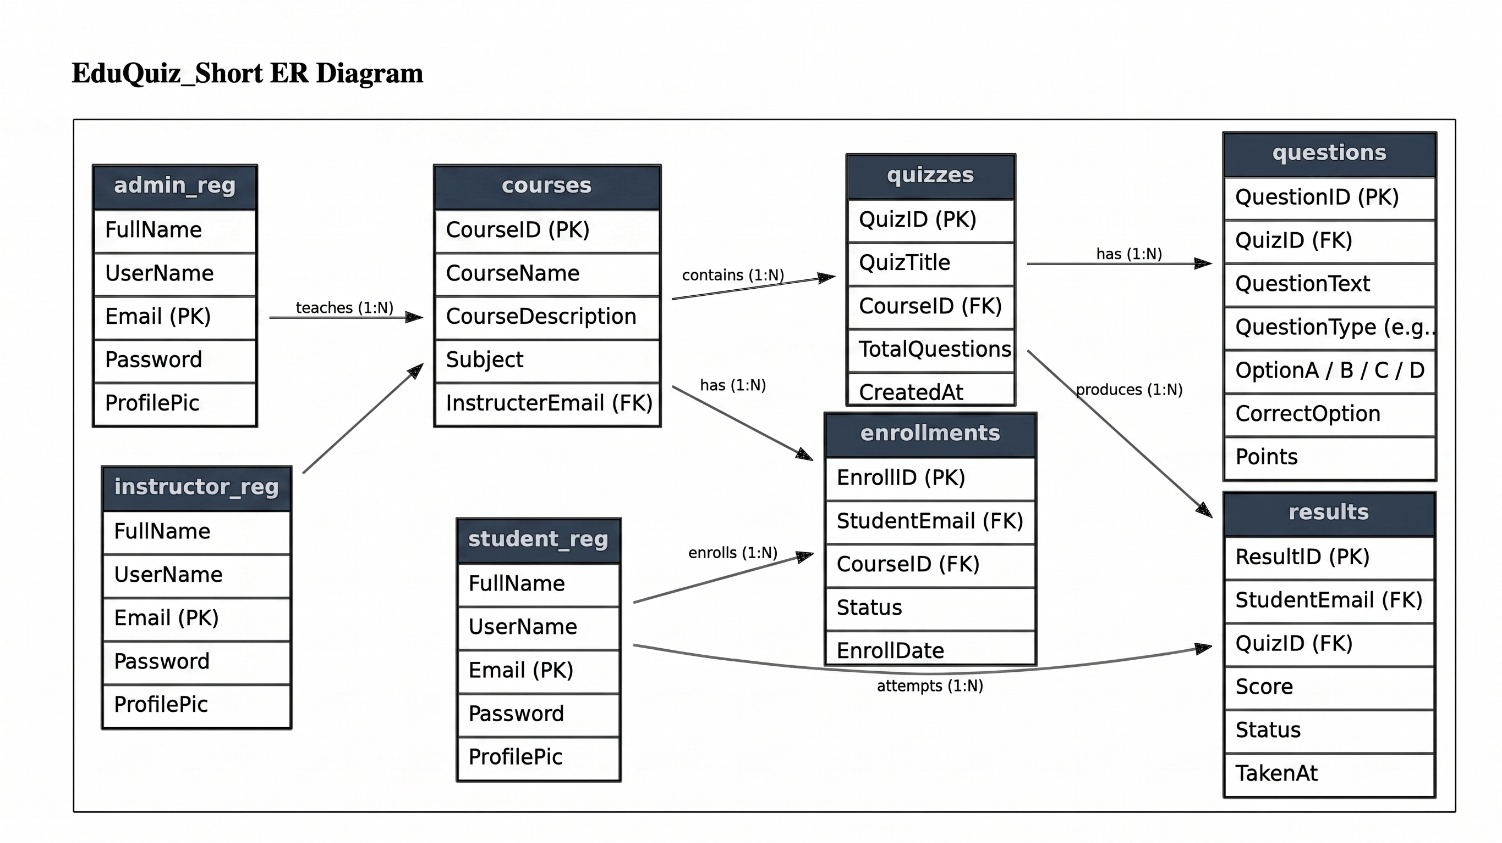
\includegraphics[width=0.92\textwidth]{figures/er_diagram.jpeg}}
\end{center}

\heading{Use Case Diagram}
\vspace{4pt}
\begin{center}
\fbox{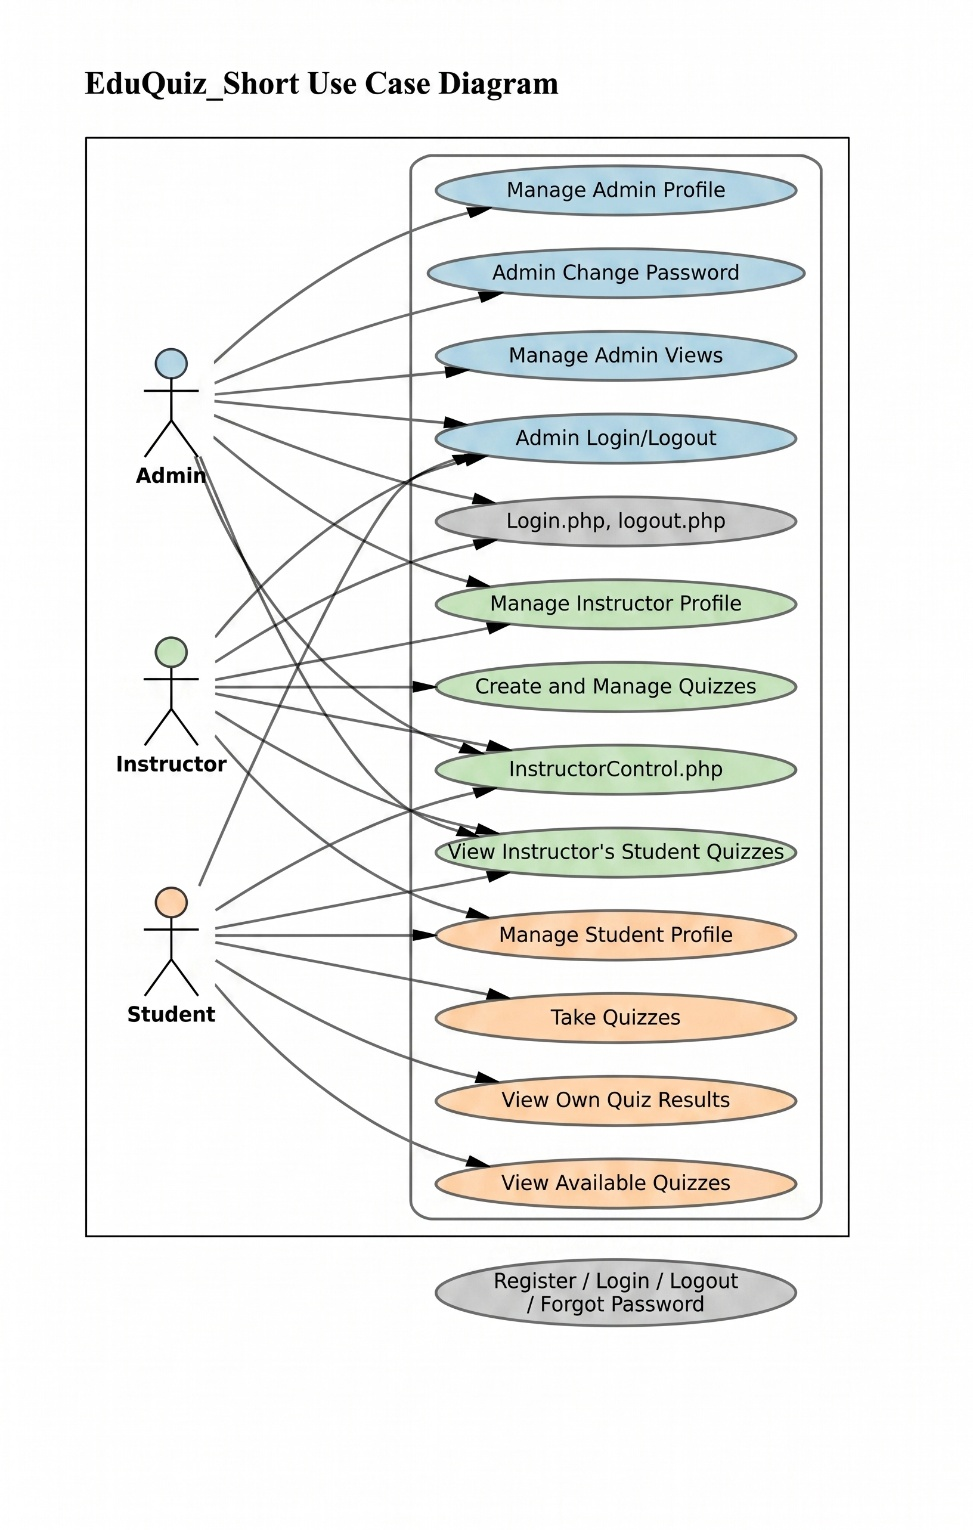
\includegraphics[height=0.52\textheight]{figures/use_case_diagram.jpeg}}
\end{center}

\newpage
% ======================= Page 3 =======================
\heading{UI (Figma/Sketch)}
\vspace{4pt}
\figtitle{Mainpage}
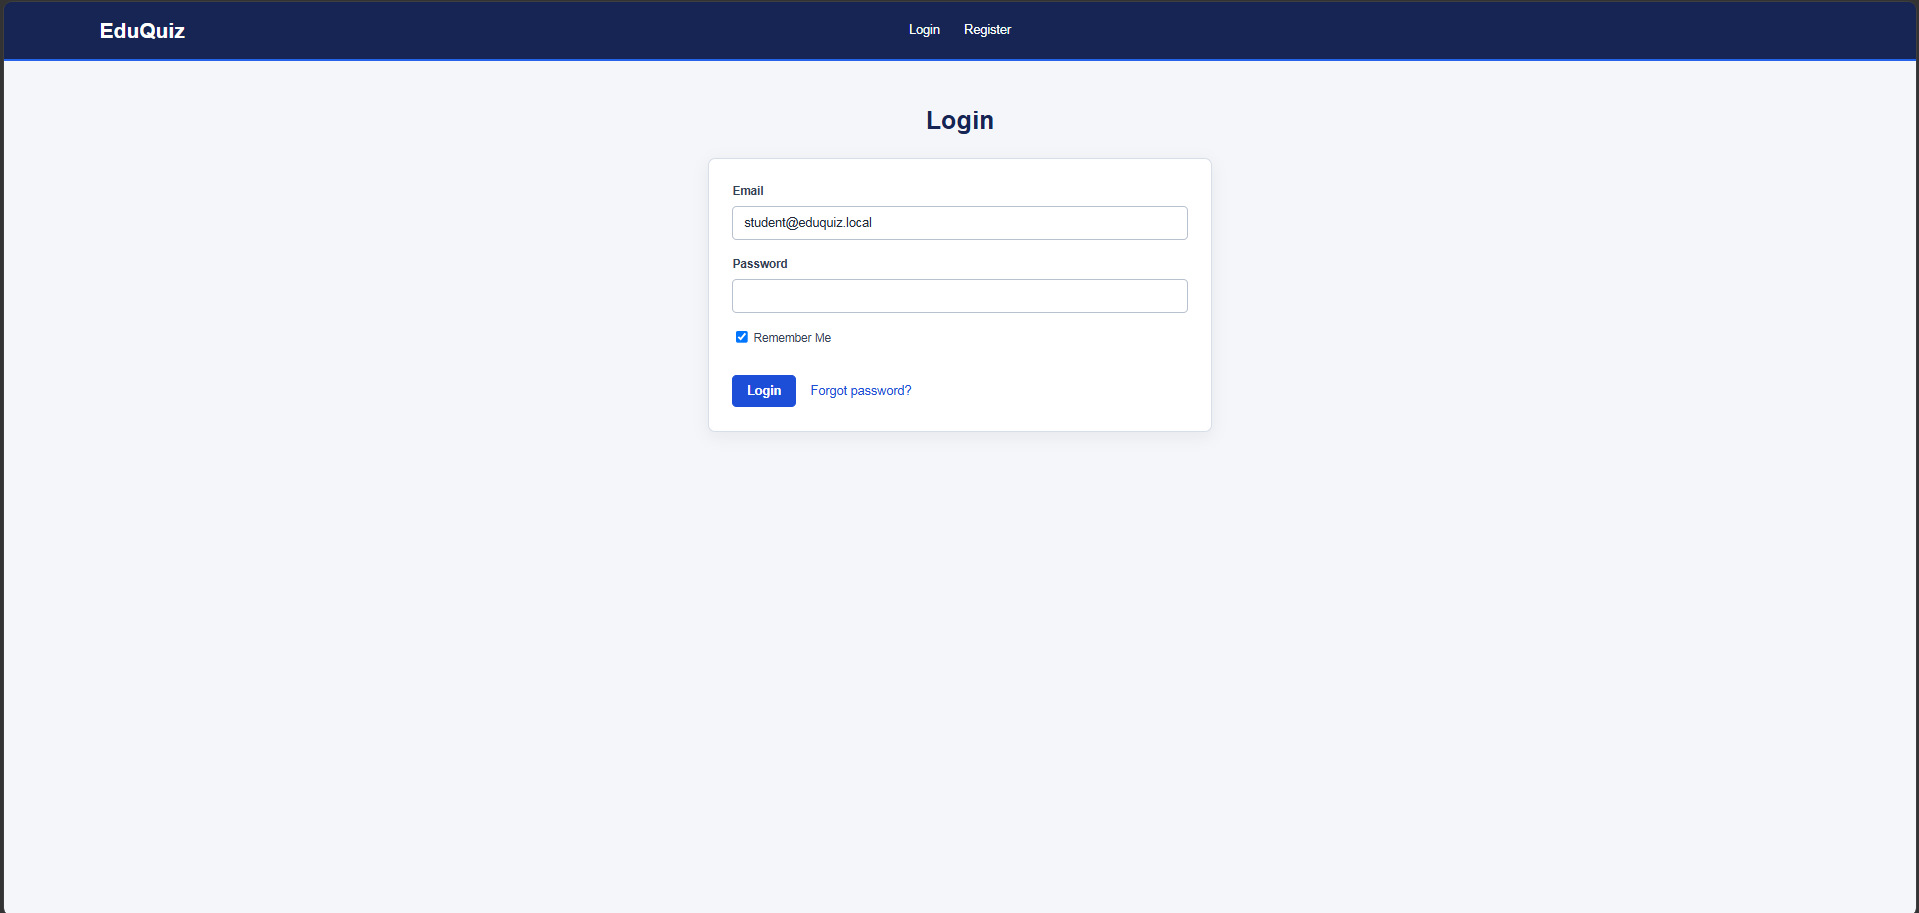
\includegraphics[width=\textwidth]{figures/ui_mainpage.png}

\vspace{14pt}
\figtitle{Admin Dashboard}
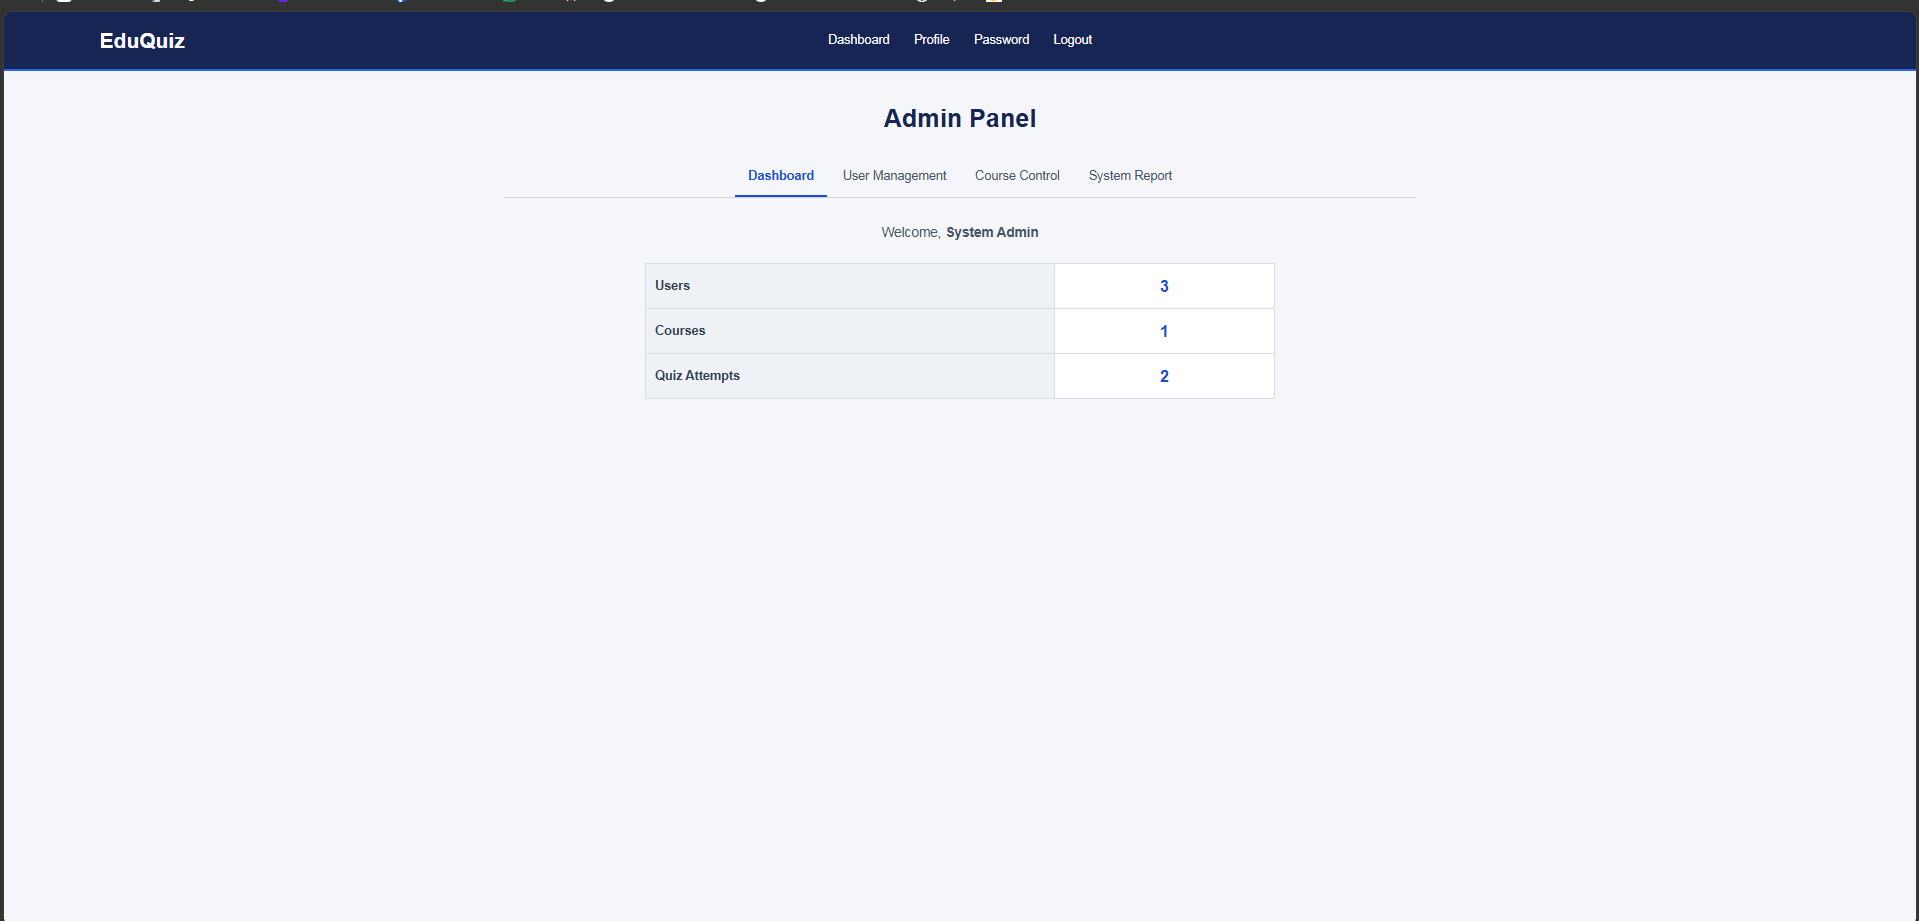
\includegraphics[width=\textwidth]{figures/ui_admin_dashboard.png}

\newpage
% ======================= Page 4 =======================
\figtitle{Instructor Dashboard}
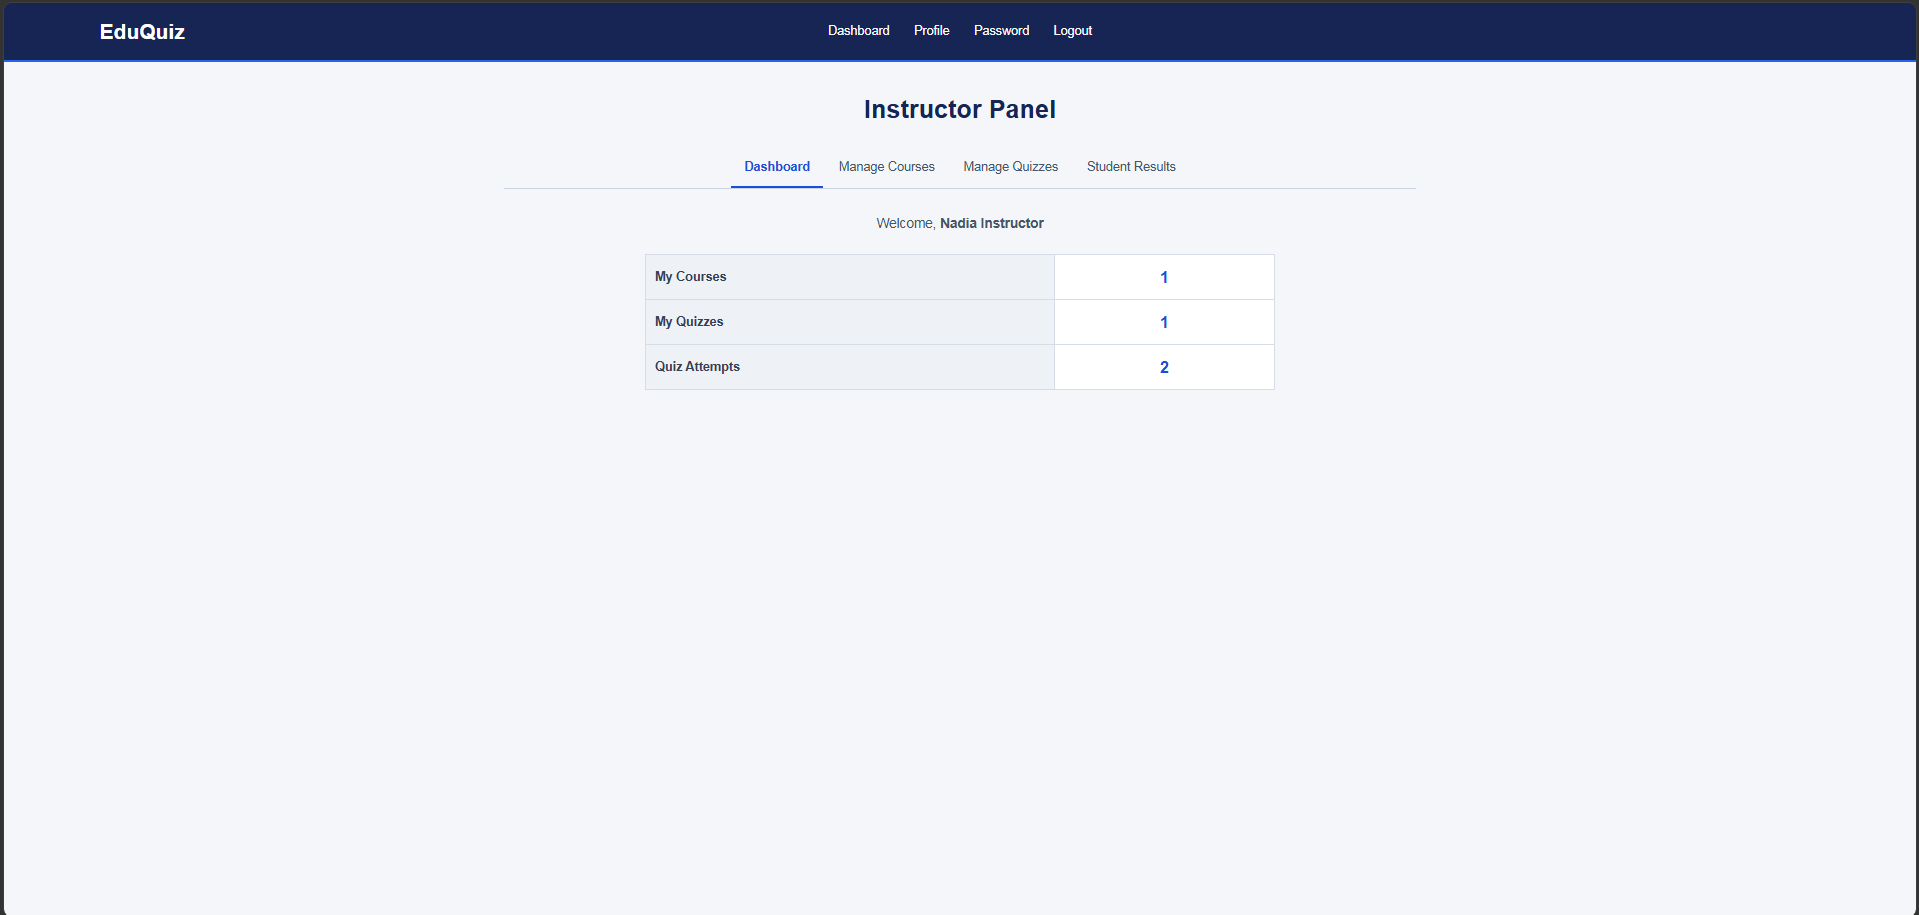
\includegraphics[width=\textwidth]{figures/ui_instructor_dashboard.png}

\vspace{14pt}
\figtitle{Student Dashboard}
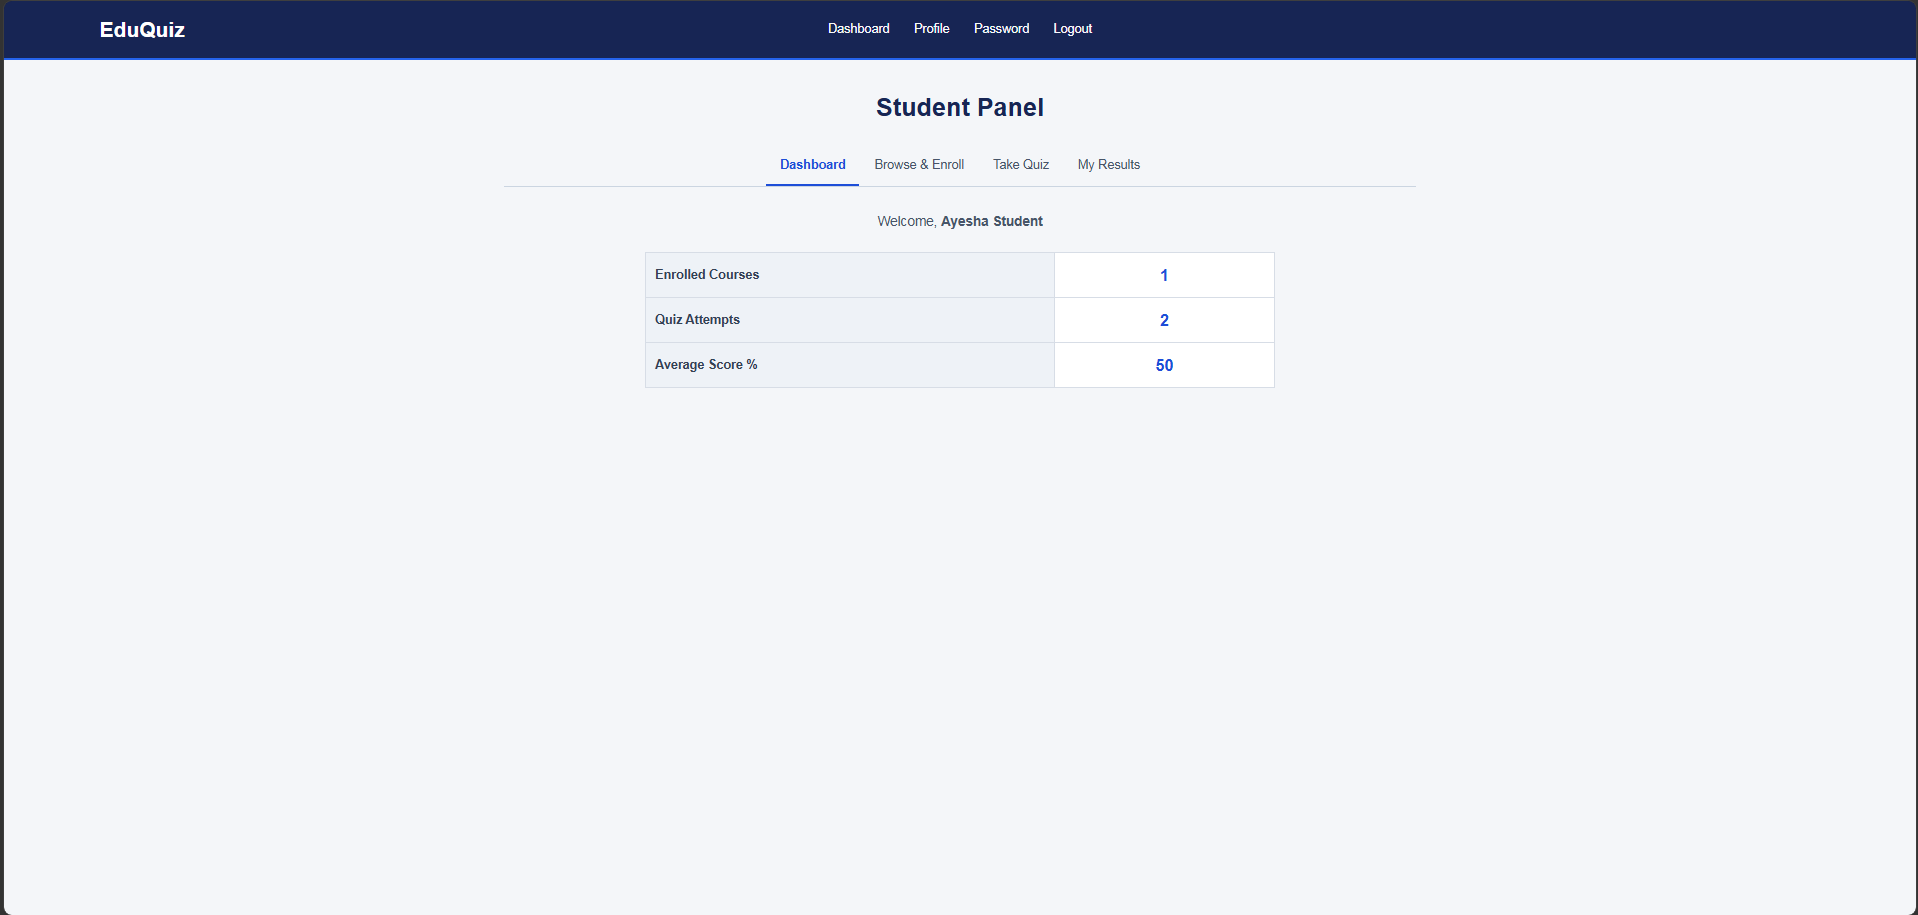
\includegraphics[width=\textwidth]{figures/ui_student_dashboard.png}

\newpage
% ======================= Page 5 =======================
\noindent\fbox{\parbox{\dimexpr\textwidth-2\fboxsep-2\fboxrule}{%
\vspace{6pt}
\textbf{Types of User}
\begin{enumerate}[leftmargin=2.2em, itemsep=0pt, topsep=4pt]
  \item \textbf{Admin}
  \item \textbf{Instructor}
  \item \textbf{Student}
\end{enumerate}

\textbf{Common Features (Available to All Users)}
\begin{itemize}[leftmargin=2.2em, itemsep=6pt, topsep=2pt]
  \item \textbf{Authentication}
  \begin{enumerate}[leftmargin=2.2em, itemsep=0pt, topsep=4pt]
    \item Login to the system
    \item Logout from the system
    \item User registration as Student or Instructor
    \item Remember Me option during login
  \end{enumerate}
  \item \textbf{Account Management}
  \begin{enumerate}[leftmargin=2.2em, itemsep=0pt, topsep=4pt]
    \item Change or reset password
    \item View profile information
    \item Edit profile information
    \item Delete account
  \end{enumerate}
  \item \textbf{Dashboard}
  \begin{enumerate}[leftmargin=2.2em, itemsep=0pt, topsep=4pt]
    \item Access a personalized dashboard after login
  \end{enumerate}
  \item \textbf{Additional Feature}
  \begin{enumerate}[leftmargin=2.2em, itemsep=0pt, topsep=4pt]
    \item AJAX-based username, email and phone availability checking during registration
  \end{enumerate}
\end{itemize}

\textbf{Specific Features by User Type}
\begin{itemize}[leftmargin=2.2em, itemsep=6pt, topsep=2pt]
  \item \textbf{Features of Admin}
  \begin{enumerate}[leftmargin=2.2em, itemsep=0pt, topsep=4pt]
    \item Manage Student and Instructor accounts, including viewing, activating/deactivating, and deleting users.
    \item View and manage courses available in the system.
    \item View system-wide statistics such as students, instructors, courses, quizzes, and quiz attempts.
  \end{enumerate}
  \item \textbf{Features of Instructor}
  \begin{enumerate}[leftmargin=2.2em, itemsep=0pt, topsep=4pt]
    \item Create and manage their own courses.
    \item Create multiple-choice quizzes and questions for courses, and see the questions of each quiz.
    \item View student quiz results, scores, and pass/fail status (pass mark: 40\%).
  \end{enumerate}
  \item \textbf{Features of Student}
  \begin{enumerate}[leftmargin=2.2em, itemsep=0pt, topsep=4pt]
    \item Browse available courses and enroll in them.
    \item Attempt multiple-choice quizzes for enrolled courses.
    \item View enrolled courses, quiz attempts, scores, average performance, and previous results.
  \end{enumerate}
\end{itemize}
\vspace{6pt}}}

\end{document}
